\section{Experimental Results}
\vspace*{-\baselineskip}
\subsection{The Nature of a Realistic Time Series}
The primary difficulty experienced in testing was an unknown aspect of time series themselves.
Originally the test problem was a very simple one-dimensional sine wave, with only a simple slope function for an operator, and with the classification task of deciding if the next point will be up or down from the current point.
This appears as if it were a trivial problem, and indeed a high degree of accuracy can be achieved with only two very simple rules:
if the previous point is below the current one then the next point will be above;
otherwise the next point will be below the current point.

This approach will not work in general.
There are several distinct types of time series, such as: up-trending, down-trending, steady, periodic, up-step, down-step, hills, and valleys.
Real-world time series are comprised of several of the characteristics from each type, and any system that would be capable of operating on a real-world time series would need to be able to handle all of the different types simultaneously.
The problem is that a simple slope operator is only capable of learning time series that are primarily linear, and a periodic time series such as the sine wave requires entirely different operators.

\subsection{The Simplistic Increasing/Decreasing Tests}
The original test time series was a sine wave, which is a perfect example of a periodic function, but the simple slope operator is only capable of learning linear time series data.
The new tests were designed with this in mind, and is actually a closer match to the appearance of real market data.

The first new test was simply a randomly chosen slope for a line, either upward or downward;
the classification question is still whether or not the next point will be above or below the current one; this was very quickly optimally learned by the system.

\enlargethispage{2\baselineskip}
In the second simple test, the series is randomly selected to be either upward or downward for a random number of time steps, with a randomly chosen slope, over and over again with completely different random elements each time.
This was also very quickly optimally learned by the system.

The third simple test added random noise to the second test;
TSC would typically optimally learn this problem within 1,000 to 2,000 time steps.

The fourth simple test randomly switched the direction of the time step with a certain probability.
This, as well, was optimally learned within 1,000 to 2,000 time steps.
This test would superficially resemble a traded entity, so it is of particular interest.
What is shown in Figures~4.1 and 4.2 is a typical run under this test, with a probability of exploration of 0.35 and a probability of random misdirection of 0.1;
% XXX: This is doing 4.2 for both figures for some reason.
%What is shown in Figures~\ref{fig:inde4plot} and \ref{fig:inde4perf} is a typical run under this test, with a probability of exploration of 0.35 and a probability of random misdirection of 0.1;
this would imply a best-case eventual accuracy of:
\[1 - \frac{0.35}{2} -0.1 = 0.725\]
or 72.5\%, which eventually appears.

\begin{figure}
%GNUPLOT: LaTeX picture with Postscript
\begin{picture}(0,0)%
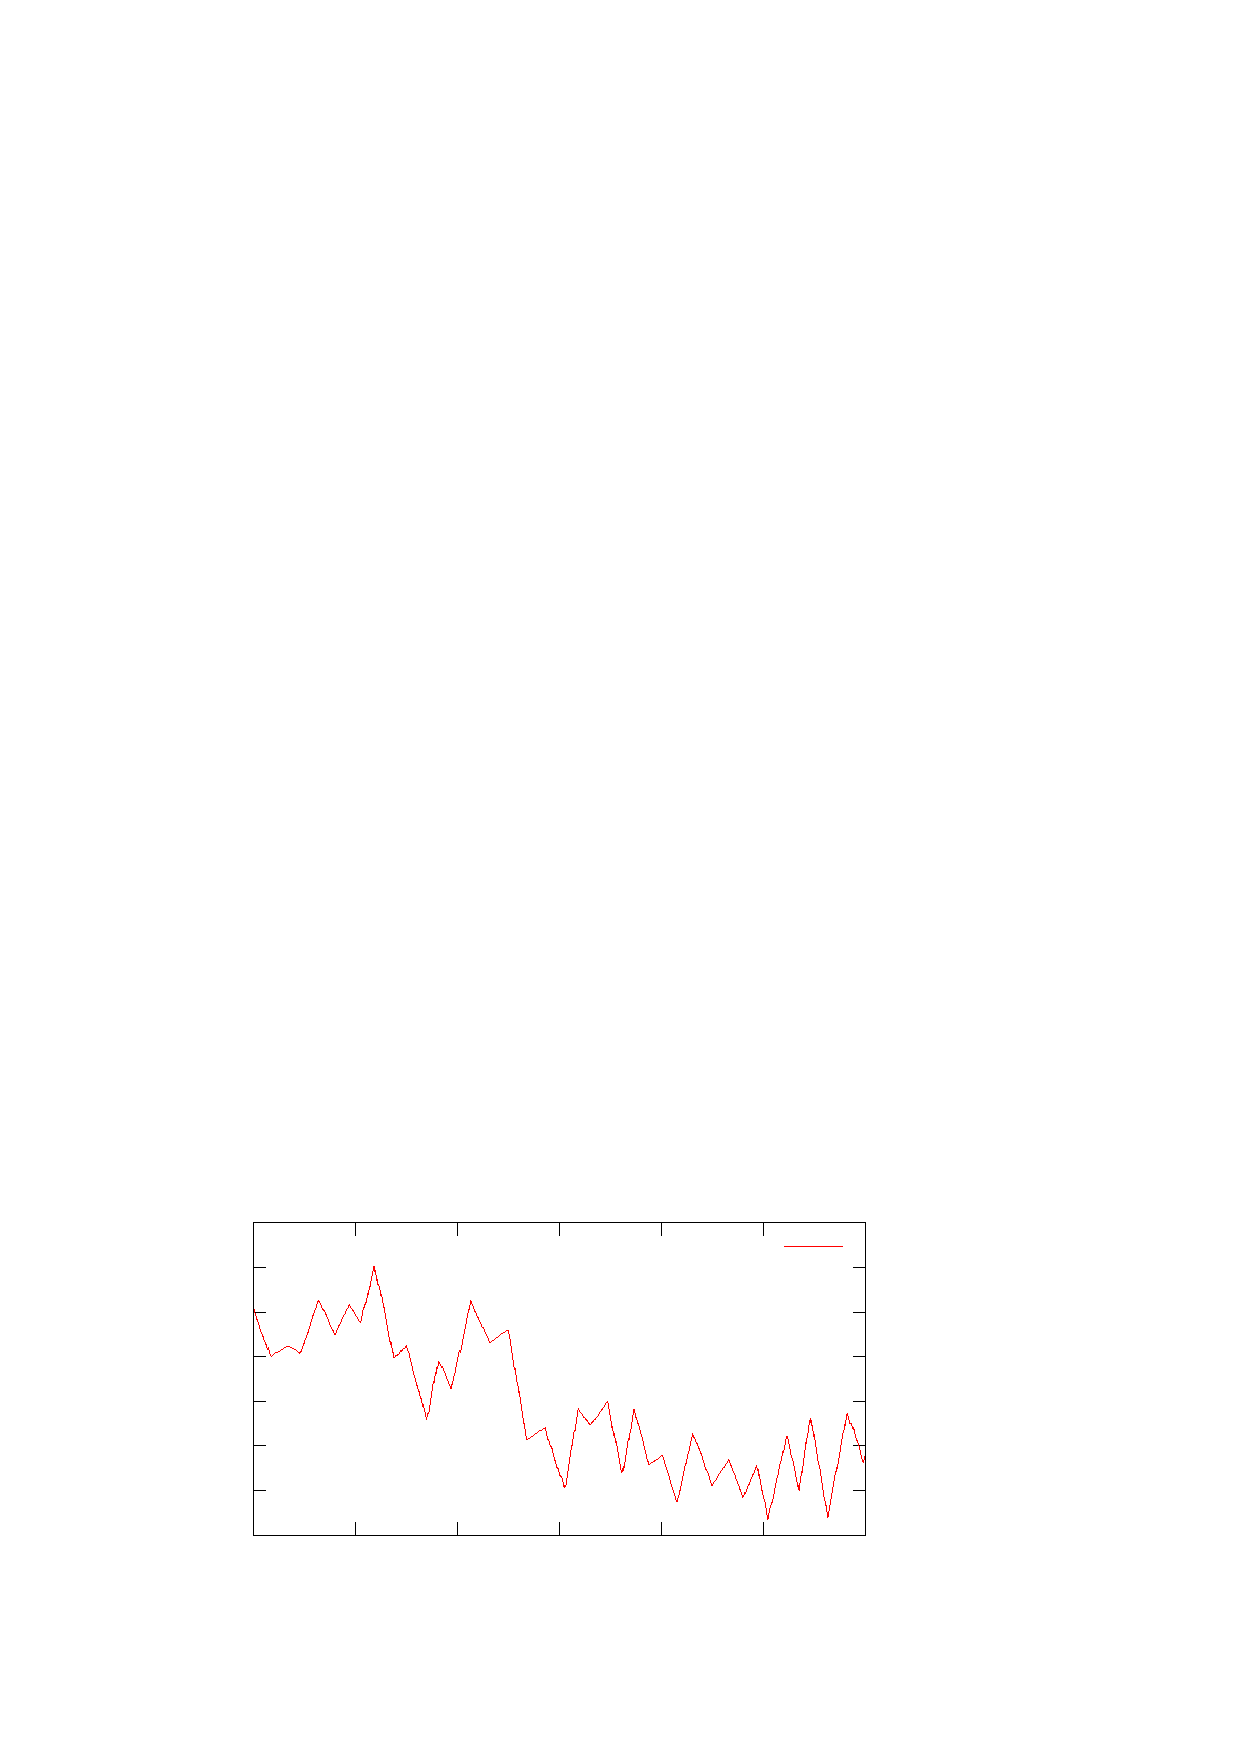
\includegraphics{inde-values}%
\end{picture}%
\begingroup
\setlength{\unitlength}{0.0200bp}%
\begin{picture}(18000,10800)(0,0)%
\put(2200,1650){\makebox(0,0)[r]{\strut{}-250}}%
\put(2200,2721){\makebox(0,0)[r]{\strut{}-200}}%
\put(2200,3793){\makebox(0,0)[r]{\strut{}-150}}%
\put(2200,4864){\makebox(0,0)[r]{\strut{}-100}}%
\put(2200,5936){\makebox(0,0)[r]{\strut{}-50}}%
\put(2200,7007){\makebox(0,0)[r]{\strut{} 0}}%
\put(2200,8079){\makebox(0,0)[r]{\strut{} 50}}%
\put(2200,9150){\makebox(0,0)[r]{\strut{} 100}}%
\put(2475,1100){\makebox(0,0){\strut{} 0}}%
\put(4925,1100){\makebox(0,0){\strut{} 500}}%
\put(7375,1100){\makebox(0,0){\strut{} 1000}}%
\put(9825,1100){\makebox(0,0){\strut{} 1500}}%
\put(12275,1100){\makebox(0,0){\strut{} 2000}}%
\put(14725,1100){\makebox(0,0){\strut{} 2500}}%
\put(17175,1100){\makebox(0,0){\strut{} 3000}}%
\put(550,5400){\rotatebox{90}{\makebox(0,0){\strut{}value}}}%
\put(9825,275){\makebox(0,0){\strut{}time step}}%
\put(9825,9975){\makebox(0,0){\strut{}increasing/decreasing method 4 sample plot}}%
\put(14950,8575){\makebox(0,0)[r]{\strut{}"inde-values.data"}}%
\end{picture}%
\endgroup
\endinput

\label{fig:inde4plot}
\caption{Increasing/decreasing method 4 sample plot.}
\end{figure}

\begin{figure}
%GNUPLOT: LaTeX picture with Postscript
\begin{picture}(0,0)%
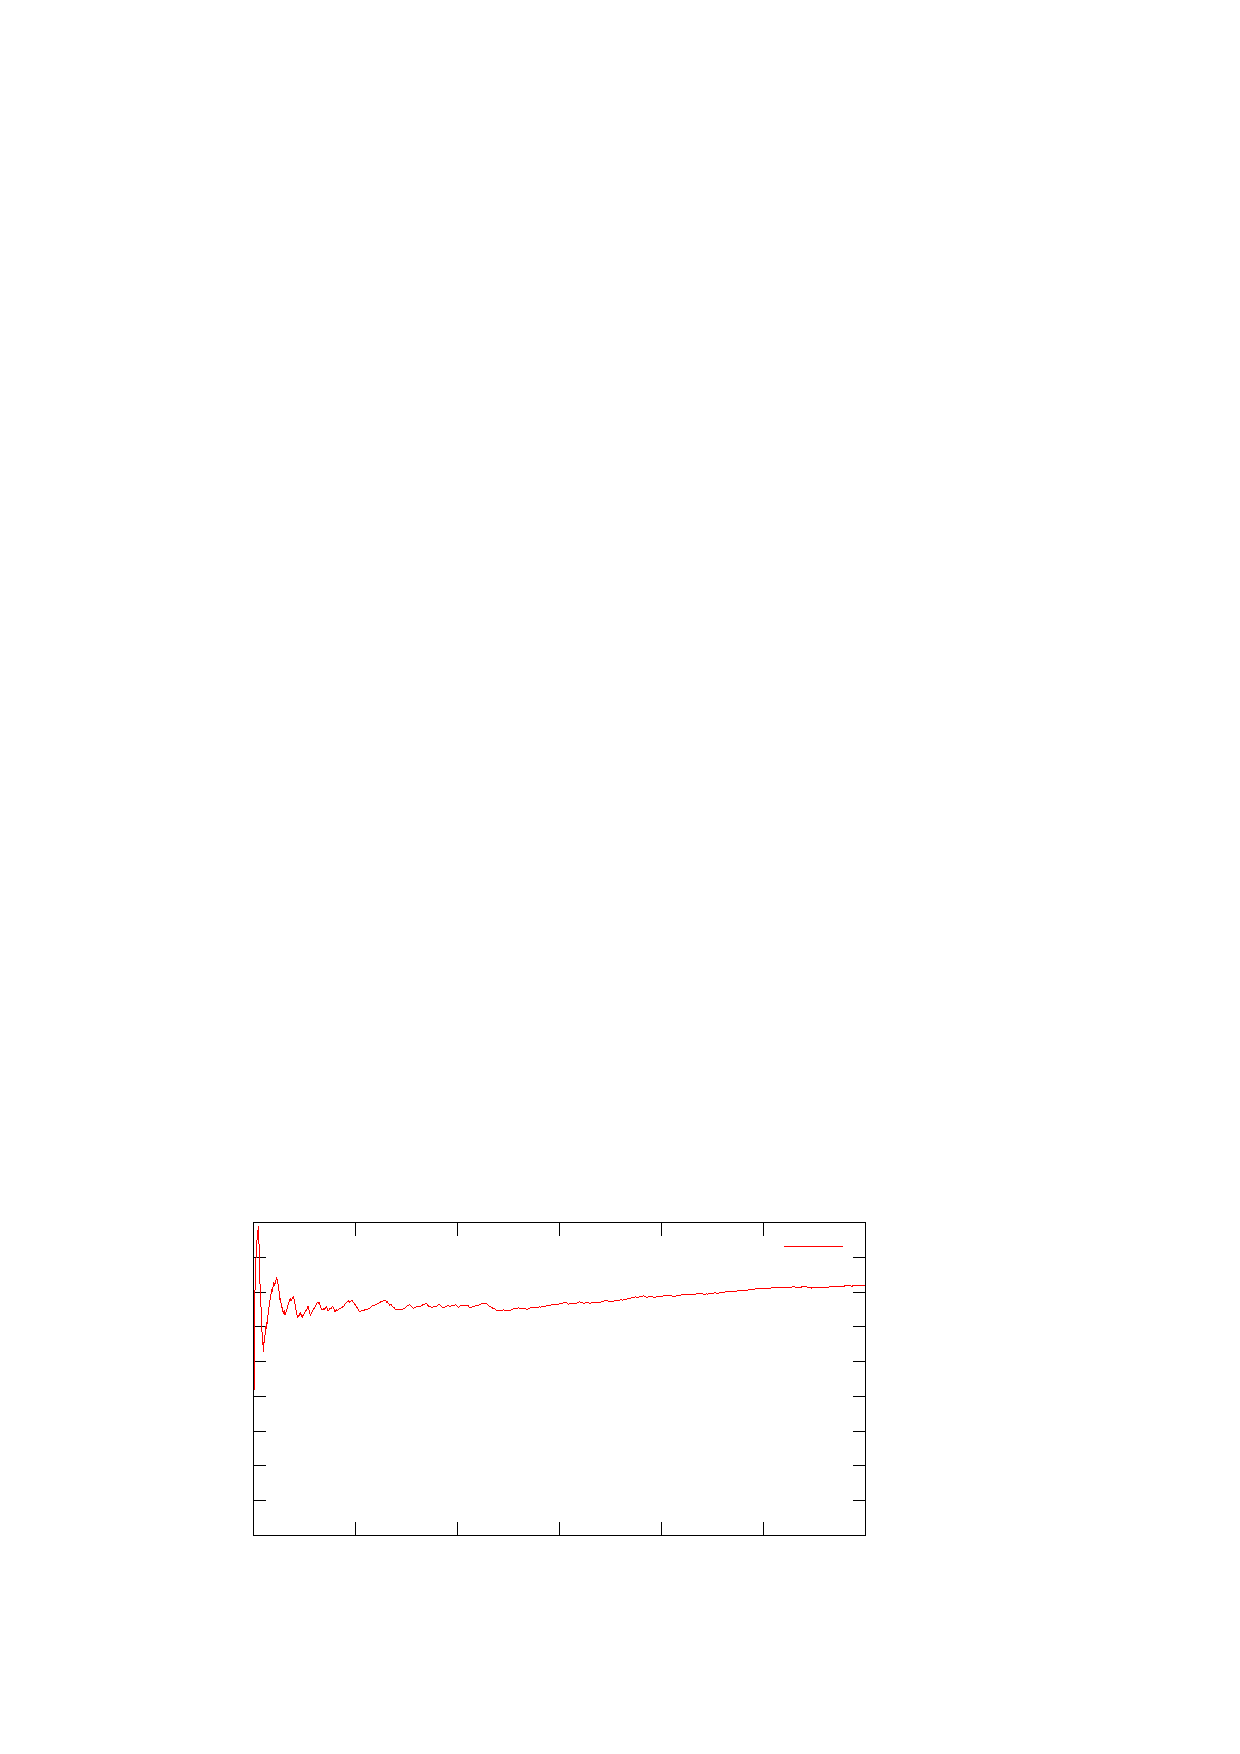
\includegraphics{inde-hist}%
\end{picture}%
\begingroup
\setlength{\unitlength}{0.0200bp}%
\begin{picture}(18000,10800)(0,0)%
\put(2200,1650){\makebox(0,0)[r]{\strut{} 0}}%
\put(2200,2483){\makebox(0,0)[r]{\strut{} 0.1}}%
\put(2200,3317){\makebox(0,0)[r]{\strut{} 0.2}}%
\put(2200,4150){\makebox(0,0)[r]{\strut{} 0.3}}%
\put(2200,4983){\makebox(0,0)[r]{\strut{} 0.4}}%
\put(2200,5817){\makebox(0,0)[r]{\strut{} 0.5}}%
\put(2200,6650){\makebox(0,0)[r]{\strut{} 0.6}}%
\put(2200,7483){\makebox(0,0)[r]{\strut{} 0.7}}%
\put(2200,8317){\makebox(0,0)[r]{\strut{} 0.8}}%
\put(2200,9150){\makebox(0,0)[r]{\strut{} 0.9}}%
\put(2475,1100){\makebox(0,0){\strut{} 0}}%
\put(4925,1100){\makebox(0,0){\strut{} 500}}%
\put(7375,1100){\makebox(0,0){\strut{} 1000}}%
\put(9825,1100){\makebox(0,0){\strut{} 1500}}%
\put(12275,1100){\makebox(0,0){\strut{} 2000}}%
\put(14725,1100){\makebox(0,0){\strut{} 2500}}%
\put(17175,1100){\makebox(0,0){\strut{} 3000}}%
\put(550,5400){\rotatebox{90}{\makebox(0,0){\strut{}accuracy}}}%
\put(9825,275){\makebox(0,0){\strut{}time step}}%
\put(9825,9975){\makebox(0,0){\strut{}increasing/decreasing method 4 sample performance}}%
\put(14950,8575){\makebox(0,0)[r]{\strut{}"inde-hist.data"}}%
\end{picture}%
\endgroup
\endinput

\label{fig:inde4perf}
\caption{Increasing/decreasing method 4 sample performance.}
\end{figure}

\subsection{The Stock Market}
\newcommand{\DJI}{\textasciicircum DJI}
We experimentally determined many of the parameters that are best for use on the stock market.
We used actual historical data of the Dow Jones Industrial Average (\DJI), with daily trading data starting on August 20, 1990, with data ending on August 18, 2006.
The data was gathered from Yahoo! Finance.
The first 100 data points of the time series were skipped, allowing for historical data that far back even in the very first day of simulated data, causing an actual start of analysis of January 11, 1991.
In each of these experiments, a statistical sample of at least 30 runs was gathered, each run going on for 1,500 simulated trading days (2,167 actual days, 5.93 years), for an end of December 16, 1996.
At each trading day the stock was given the option to either put all of its resources into the \DJI\ or into a bank account yielding roughly 4\% per annum.
The system initially had \$1,000,000.00.

In these trials we report:
\begin{enumerate}
\item the trial number,
\item the number of correct actions,
\item the percentage of correct actions,
\item the final financial return,
\item the ratio of the final financial return to that of the buy-and-hold strategy,
\item and the percentage returned per annum.
\end{enumerate}
We will use the buy-and-hold (B\&H) strategy as our primary performance benchmark.
In this strategy, the stock is purchased outright, and then the money is just left in the stock for the entire duration of the experiment.

\newenvironment{cgoreErt}[2]
{\begin{center}
   \begin{longtable}{|c|lrrlr|}
      \caption{#1}\label{#2}\remline\\
      \hline
      --- & \textbf{correct} & \textbf{\% correct} & \textbf{returns} & \textbf{B\&H ratio} & \textbf{\%pa}\\
      \hline
      B\&H & 806 & 53.733\% & \$2,745,309.50 & 1.0 & 18.54\%pa\\
      \hline
   \endfirsthead}
{\\ \hline\end{longtable}\end{center}}

Our initial parameters are listed in Table~\ref{tab:initial-parameters}, and were chosen by general trial and error throughout the software development process.

\begin{table}
\caption{Initial parameters for the TSC.}
\label{tab:initial-parameters}
\begin{tabular}{|r|l|}
   \hline
   \textbf{parameter} & \textbf{value} \\
   \hline
   max environment condition length & 10 \\
   valid operations & simple slope \\
   valid fields & closing price, opening price, and trading volume \\
   max total numerosity, $N$ & 400 \\
   learning rate, $\beta$ & 0.2 \\
   discount factor, $\gamma$ & 0.71 \\
   GA threshold, $\theta_{GA}$ & 25 \\
   equal error threshold, $\epsilon_0$ & 20.0 \\
   multiplier parameter, $\alpha$ & 0.1 \\
   crossover probability, $\chi$ & 0.8 \\
   mutation probability, $\mu$ & 0.04 \\
   exploration probability, $P_{explr}$ & 0.2 \\
   fitness fraction threshold, $\delta$ & 0.1 \\
   covering probability, $P_\#$ & 0.33 \\
   initial prediction, $p_I$ & 10.0 \\
   initial prediction error, $\epsilon_I$ & 0.0 \\
   initial fitness, $F_I$ & 0.01\\
   \hline
\end{tabular}
\end{table}

\subsubsection{Reward Methods}
Several different possible reward methods for use in the stock market were considered, and we analyzed their relative performance.
We refer to these different reward methods as $a_1$, $a_2$, $b$, $c$, $d_{opt}$, and $d_{pess}$.

Reward method $a_1$ is very simple:
\begin{algorithmic}[1]
\IF{the correct action is taken}
   \RETURN a reward of 1,000.
\ELSE
   \RETURN a reward of 0,
\ENDIF
\end{algorithmic}

It had the results as described in Table~\ref{tab:reward-a1} over 36 trials.

\begin{cgoreErt}{TSC results for reward method $a_1$.}{tab:reward-a1}
arith mean & 754 & 50.256\% & \$1,853,080.30 & 0.67500 & 10.96\%pa \\
std dev & 22.3 & 1.489\% & \$333,964.25 & 0.12165 & 1.98\%pa \\
max & 797 & 53.133\% & \$2,527,462.80 & 0.92065 & 16.91\%pa \\
min & 697 & 46.467\% & \$1,117,451.00 & 0.40704 & 1.89\%pa
\end{cgoreErt}

Reward method $a_2$ is almost identical to $a_1$:
\begin{algorithmic}[1]
\IF{the correct action is taken}
   \RETURN a reward of 1,000.
\ELSE
   \RETURN a reward of -200.
\ENDIF
\end{algorithmic}

It had the results as described in Table~\ref{tab:reward-a2} over 44 trials.

\begin{cgoreErt}{TSC results for reward method $a_2$.}{tab:reward-a2}
arith mean & 748 & 49.867\% & \$1,863,365.60 & 0.67875 & 11.06\%pa \\
std dev & 23.4 & 1.557\% & \$294,466.10 & 0.10726 & 1.75\%pa \\
max & 790 & 52.667\% & \$2,571,187.50 & 0.93657 & 17.25\%pa \\
min & 693 & 46.2\% & \$1,358,889.10 & 0.49499 & 5.31\%pa
\end{cgoreErt}

Reward method $b$ offers slightly more incentive for good-performing rules:
\begin{algorithmic}[1]
\LETARROW{$\$_{ratio}$, the money ratio} $\frac{\$_{t+1}}{\$_t}$, the ratio of the money the classifier has immediately one time-step in the future to the money it currently has.
\IF{$\$_{ratio} > 1.005$}
   \RETURN a reward of 1,000.
\ELSE
   \RETURN a reward of 0.
\ENDIF
\end{algorithmic}

It had the results as described in Table~\ref{tab:reward-b} over 57 trials.

\begin{cgoreErt}{TSC results for reward method $b$.}{tab:reward-b}
arith mean & 750 & 49.992\% & \$1,792,041.90 & 0.65276 & 10.33\%pa \\
std dev & 27.9\% & 1.8631344 & \$378,179.50 & 0.13775 & 2.18\%pa \\
max & 815 & 54.333\% & \$2,820,059.80 & 1.02723 & 19.09\%pa \\
min & 692 & 46.133\% & \$1,219,942.60 & 0.44437 & 3.41\%pa
\end{cgoreErt}

Reward method $c$ tries to scale the reward:
\begin{algorithmic}[1]
\LET $\$_{ratio}$ be the money ratio as previously defined.
\LETARROW{$m$} 1000, a multiplier.
\LETARROW{$e$} 2, an exponent.
\LETARROW{$s$} 1.015, a threshold term.
\RETURN $m \cdot (\$_{ratio}-s)^e$
\end{algorithmic}

It had the results as described in Table~\ref{tab:reward-c} over 30 trials.

\begin{cgoreErt}{TSC results for reward method $c$.}{tab:reward-c}
arith mean  & 747 & 49.791\% & \$1,795,971.30 & 0.65420 & 10.37\%pa \\
std dev & 20.2 & 1.345\% & \$300,842.88 & 0.10958 & 1.74\%pa \\
max & 790 & 52.667\% & \$2,407,121.50 & 0.87681 & 15.95\%pa \\
min & 702 & 46.8\% & \$1,340,345.30 & 0.48823 & 5.07\%pa
\end{cgoreErt}

\newpage
Reward method $d$ is slightly more complex than the rest:
\begin{algorithmic}[1]
\INPUT $cu$, the amount of reward if the classifier is correct on an up day.
\INPUT $cd$, the amount of reward if the classifier is correct on an down day.
\INPUT $iu$, the amount of reward if the classifier is incorrect on an up day.
\INPUT $id$, the amount of reward if the classifier is incorrect on an down day.
\COMMENT{Days that are not up are viewed as down days here.}
\IF{the classifier has chosen the correct action $\land$ it is an up day}
   \RETURN $cu$.
\ELSIF{the classifier has chosen the correct action $\land$ it is a down day}
   \RETURN $cd$.
\ELSIF{the classifier has chosen the incorrect action $\land$ it is an up day}
   \RETURN $iu$.
\ELSIF{the classifier has chosen the incorrect action $\land$ it is a down day}
   \RETURN $id$.
\ENDIF
\end{algorithmic}
From this we have the two reward methods $d_{opt}$, which is optimistic, and $d_{pess}$, which is pessimistic.

Reward method $d_{opt}$ calls $d$ with the values of $cu=1000, cd=750, iu=0, id=200$.
It had the results as described in Table~\ref{tab:reward-dopt} over 45 trials.

\begin{cgoreErt}{TSC results for reward method $d_{opt}$.}{tab:reward-dopt}
arith mean & 728 & 48.526\% & \$1,624,189.40 & 0.59162 & 8.52\%pa \\
std dev & 22.2 & 1.477\% & \$223,009.56 & 0.08123 & 1.17\%pa \\
max & 786 & 52.4\% & \$2,122,616.30 & 0.77318 & 13.52\%pa \\
min & 689 & 45.933\% & \$1,163,151.90 & 0.42369 & 2.58\%pa
\end{cgoreErt}

Reward method $d_{pess}$ calls $d$ with the values of $cu=750, cd=1000, iu=200, id=0$.
It had the results as described in Table~\ref{tab:reward-dpess} over 45 trials.

\begin{cgoreErt}{TSC results for reward method $d_{pess}$.}{tab:reward-dpess}
arith mean & 728 & 48.526\% & \$1,624,189.40 & 0.59162 & 8.52\%pa \\
std dev & 22.2\% & 1.477 & \$223,009.56 & 0.08123 & 1.17\%pa \\
max & 786 & 52.4\% & \$2,122,616.30 & 0.77318 & 13.52\%pa \\
min & 689 & 45.933\% & \$1,163,151.90 & 0.42369 & 2.58\%pa
\end{cgoreErt}

From these experiments we see that the $a$ methods are the best performing, although there is no effective difference between the performance of $a_1$ and $a_2$: this is because the scaling of the reward should not effect the outcome of the reward method at all.
We arbitrarily choose of the two to employ $a_2$ for the remaining experiments.


\subsubsection{GA Thresholds}
After deciding on $a_2$ as the best reward method and keeping it for the rest of these tests, we turn our attention to optimizing the GA threshold $\theta_{GA}$, which is described earlier in \S\ref{sec:ga-threshold}.
We chose to look at the possible values for this parameter of 25,  35, 45, and 50.

A GA threshold of 25 was used in the previous situation, so we can borrow the results from that $a_2$ run; refer to Table~\ref{tab:reward-a2}.

For a GA threshold value of 35, we observed the results as described in Table~\ref{tab:gathreshold35} over 30 trials.

\enlargethispage{2\baselineskip}
\begin{cgoreErt}{TSC results for a GA threshold of 35.}{tab:gathreshold35}
arith mean & 759 & 50.571\% & \$1,874,746.50 & 0.68289 & 11.17\%pa \\
std dev & 22.7 & 1.513\% & \$315,092.60 & 0.11477 & 1.88\%pa \\
max & 806 & 53.733\% & \$2,627,517.80 & 0.95709 & 17.68\%pa \\
min & 719 & 47.933\% & \$1,346,346.10 & 0.49042 & 5.14\%pa
\end{cgoreErt}

For a GA threshold value of 45, we observed the results as described in Table~\ref{tab:gathreshold45} over 31 trials.

\begin{cgoreErt}{TSC results for a GA threshold of 45.}{tab:gathreshold45}
arith mean & 760  & 50.688\% & \$1,881,119.10 & 0.68521 & 11.24\%pa \\
std dev    & 25.6 &  1.706\% &   \$217,843.06 & 0.07935 & 1.30\%pa \\
max        & 816  & 54.4\%   & \$2,297,796.00 & 0.83699 & 15.05\%pa \\
min        & 699  & 46.6\%   & \$1,250,916.30 & 0.45566 & 3.85\%pa
\end{cgoreErt}

For a GA threshold value of 50, we observed the results as described in Table~\ref{tab:gathreshold50} over 30 trials.

\begin{cgoreErt}{TSC results for a GA threshold of 50.}{tab:gathreshold50}
arith mean & 763 & 50.891\% & \$1,885,079.90 & 0.68665 & 11.28\%pa \\
std dev & 21.1 & 1.405\% & \$293,885.56 & 0.10705 & 1.76\%pa \\
max & 808 & 53.867\% & \$2,425,741.30 & 0.88359 & 16.10\%pa \\
min & 713 & 47.533\% & \$1,329,746.00 & 0.48437 & 4.91\%pa
\end{cgoreErt}

There was no significant effect on the results of the algorithm based on the GA threshold: all of the other means fall well within $1\over4$ of a standard deviation relative to the initial value of $\theta_{GA} = 25$, so we will employ that value for all remaining experiments.


\subsubsection{Crossover Probabilities}
After deciding on the correct reward method and the correct GA threshold, using those results, we investigated the crossover probability, which is described earlier in \S\ref{sec:crossover-probability}.
We chose to look at 0.5, 0.6, 0.7, 0.8, and 0.9.

For a crossover probability of $\chi = 0.3$, we obtained the results as described in Table~\ref{tab:chi0.3} over 33 trials.

\begin{cgoreErt}{TSC results for $\chi=0.3$.}{tab:chi0.3}
arith mean & 755 & 50.358\% & \$1,862,015.40 & 0.67825 & 11.05\%pa \\
std dev & 24.3 & 1.621\% & \$213,367.14 & 0.07772 & 1.27\%pa \\
max & 829 & 55.267\% & \$2,354,066.50 & 0.85749 & 15.52\%pa \\
min & 712 & 47.467\% & \$1,313,611.90 & 0.47849 & 4.71\%pa
\end{cgoreErt}

For a crossover probability of $\chi = 0.5$, we obtained the results as described in Table~\ref{tab:chi0.5} over 31 trials.

\begin{cgoreErt}{TSC results for $\chi=0.5$.}{tab:chi0.5}
arith mean & 754 & 50.275\% & \$1,882,082.30 & 0.68556 & 11.25\%pa \\
std dev & 24.9 & 1.662\% & \$265,281.13 & 0.09663 & 1.59\%pa \\
max & 799 & 53.267\% & \$2,426,894.30 & 0.88401 & 16.11\%pa \\
min & 717 & 47.8 & \$1,354,985.40 & 0.49356 & 5.25\%pa
\end{cgoreErt}

For a crossover probability of $\chi = 0.7$, we obtained the results as described in Table~\ref{tab:chi0.7} over 34 trials.

\begin{cgoreErt}{TSC results for $\chi=0.7$.}{tab:chi0.7}
arith mean & 754 & 50.275\% & \$1,884,173.30 & 0.68632 & 11.27\%pa \\
std dev & 28.9 & 1.930\% & \$258,017.90 & 0.09399 & 1.54\%pa \\
max & 809 & 53.933\% & \$2,526,742.80 & 0.92039 & 16.90\%pa \\
min & 688 & 45.867\% & \$1,264,236.40 & 0.46051 & 4.03\%pa
\end{cgoreErt}

A crossover probability of 0.8 was used in the previous situation, so we can borrow the results from the $\theta_{GA} = 25$ run; refer to Table~\ref{tab:reward-a2}.

For a crossover probability of $\chi = 0.9$, we obtained the results as described in Table~\ref{tab:chi0.9} over 39 trials.

\begin{cgoreErt}{TSC results for $\chi=0.9$.}{tab:chi0.9}
arith mean & 759 & 50.626\% & \$1,943,606.10 & 0.70797 & 11.85\% \\
std dev & 21.9 & 1.462\% & \$277,516.22 & 0.10109 & 1.69\%  \\
max & 801 & 53.400\% & \$2,399,683.00 & 0.87410 & 15.89\% \\
min & 707 & 47.133\% & \$1,419,889.40 & 0.51721 & 6.09\%
\end{cgoreErt}

We can now easily observe that a crossover probability of $\chi=0.9$ offers the best results with an arithmetic mean of 11.85\%pa, and we employ it for all of the remaining experiments.


\subsubsection{Mutation Probabilities}
Using all of our previous results, we then looked into the mutation probability, described earlier in \S\ref{sec:mutation-probability}.
We looked at values of 0.04, 0.06, 0.08, 0.10, 0.15, and 0.20.

A mutation probability $\mu=0.04$ was used in the previous situation, so we can borrow the results from the $\chi = 0.9$ run; refer to Table~\ref{tab:chi0.9}.

For a mutation probability $\mu=0.06$, we observed the results as described in Table~\ref{tab:mu0.06} over 34 trials.

\begin{cgoreErt}{TSC results for $\mu=0.06$.}{tab:mu0.06}
arith mean & 762 & 50.831\% & \$1,972,095.00 & 0.71835 & 12.13\%pa \\
std dev & 21.5 & 1.433\% & \$255,299.13 & 0.09299 & 1.57\%pa \\
max & 792 & 52.800\% & \$2,734,496.80 & 0.99606 & 18.47\%pa \\
min & 704 & 46.933\% & \$1,579,600.50 & 0.57538 & 8.01\%pa
\end{cgoreErt}

For a mutation probability $\mu=0.08$, we observed the results as described in Table~\ref{tab:mu0.08} over 39 trials.

\begin{cgoreErt}{TSC results for $\mu=0.08$.}{tab:mu0.08}
arith mean & 754 & 50.285\% & \$1,905,925.10 & 0.69425 & 11.48\%pa \\
std dev & 29.79326 & 1.986\% & \$285,127.30 & 0.10386 & 1.72\%pa \\
max & 806 & 53.733\% & \$2,421,790.30 & 0.88216 & 16.07\%pa  \\
min & 668 & 44.533\% & \$1,230,840.30 & 0.44834 & 3.56\%pa
\end{cgoreErt}

For a mutation probability $\mu=0.10$, we observed the results as described in Table~\ref{tab:mu0.10} over 36 trials.

\begin{cgoreErt}{TSC results for $\mu=0.10$.}{tab:mu0.10}
arith mean & 761 & 50.744\% & \$1,950,889.10 & 0.71063 & 11.92\%pa \\
std dev & 22.6 & 1.506\% & \$299,845.56 & 0.10922 & 1.83\%pa \\
max & 796 & 53.067\% & \$2,891,320.00 & 1.05319 & 19.59\%pa \\
min & 709 & 47.267\% & \$1,250,508.00 & 0.45551 & 3.84\%pa
\end{cgoreErt}

For a mutation probability $\mu=0.15$, we observed the results as described in Table~\ref{tab:mu0.15} over 32 trials.

\begin{cgoreErt}{TSC results for $\mu=0.15$.}{tab:mu0.15}
arith mean & 763 & 50.908\% & \$2,037,007.90 & 0.74200 & 12.74\%pa \\
std dev & 22.299\% & 1.487\% & \$320,506.80 & 0.11675 & 2.00\%pa \\
max & 804 & 53.600\% & \$2,975,396.80 & 1.08381 & 20.17\%pa \\
min & 719 & 47.933\% & \$1,406,036.50 & 0.51216 & 5.91\%pa
\end{cgoreErt}

For a mutation probability $\mu=0.20$, we observed the results as described in Table~\ref{tab:mu0.20} over 36 trials.

\enlargethispage{2\baselineskip}
\begin{cgoreErt}{TSC results for $\mu=0.20$.}{tab:mu0.20}
arith mean & 762 & 50.800\% & \$1,889,297.80 & 0.68819 & 11.42\%pa \\
std dev & 24.369835 & 1.625\% & \$232,916.92 & 0.08484 & 1.40\%pa \\
max & 803 & 53.533\% & \$2,708,086.00 & 0.98644 & 18.28\%pa \\
min & 697 & 46.467\% & \$1,502,196.10 & 0.54719 & 7.10\%pa
\end{cgoreErt}

We can now easily observe that a mutation probability of $\mu=0.15$ offers the best results with a arithmetic mean of 12.74\%pa, and we therefore use that value for all remaining experiments.


\subsubsection{Exploration Probabilities}
After this we looked at the exploration probability, which we describe in \S\ref{sec:exploration-probability}.
We investigated the possible values of 0.1, 0.2, 0.3, and 0.4, using our previous results for the rest of the parameters.

For an exploration probability of $P_{explr}=0.1$, we observed the results as described in Table~\ref{tab:pexplr0.1} over 42 trials.

\begin{cgoreErt}{TSC results for $P_{explr}=0.1$.}{tab:pexplr0.1}
arith mean & 762 & 50.795\% & \$1,849,187.80 & 0.67358 & 10.92\%pa \\
std dev & 28.9 & 1.925\% & \$233,230.42 & 0.08496 & 1.38\%pa \\
max & 810 & 54.000\% & \$2,446,262.50 & 0.89107 & 16.27\%pa \\
min & 691 & 46.067\% & \$1,210,933.40 & 0.44109 & 3.28\%pa
\end{cgoreErt}

An exploration probability of $P_{explr}=0.2$ was used in the previous situation, so we can borrow the results from the $\mu=0.15$ run; refer to Table~\ref{tab:mu0.15}.

\begin{cgoreErt}{TSC results for $P_{explr}=0.15$.}{tab:pexplr0.15}
\hline
arith mean & 763 & 50.908\% & \$2,037,007.90 & 0.74200 & 12.74\%pa \\
std dev & 22.3 & 1.487\% & \$320,506.80 & 0.11675 & 2.00\%pa \\
max & 804 & 53.600\% & \$2,975,396.80 & 1.08381 & 20.17\%pa \\
min & 719 & 47.933\% & \$1,406,036.50 & 0.51216 & 5.91\%pa
\end{cgoreErt}

For an exploration probability of $P_{explr}=0.3$, we observed the results as described in Table~\ref{tab:pexplr0.3} over 40 trials.

\begin{cgoreErt}{TSC results for $P_{explr}=0.3$.}{tab:pexplr0.3}
arith mean & 765 & 50.985\% & \$2,090,409.40 & 0.76145 & 13.23\%pa \\
std dev & 22.8 & 1.521\% & \$295,592.78 & 0.10768 & 1.87\%pa \\
max & 817 & 54.467\% & \$2,848,646.30 & 1.03764 & 19.29\%pa \\
min & 725 & 48.333\% & \$1,536,175.30 & 0.55956 & 7.50\%pa
\end{cgoreErt}

For an exploration probability of $P_{explr}=0.4$, we observed the results as described in Table~\ref{tab:pexplr0.4} over 47 trials.

\begin{cgoreErt}{TSC results for $P_{explr}=0.4$.}{tab:pexplr0.4}
arith mean & 767 & 51.119\% & \$1,950,627.60 & 0.71053 & 11.92\%pa \\
std dev & 19.5 & 1.299\% & \$196,644.44 & 0.07163 & 1.20\%pa \\
max & 806 & 53.733\% & \$2,395,224.50 & 0.87248 & 15.86\%pa \\
min & 730 & 48.667\% & \$1,637,668.40 & 0.59653 & 8.67\%pa
\end{cgoreErt}

We can now easily observe that an exploration probability of $P_{explr}=0.3$ offers the best results with an arithmetic mean of 13.23\%pa, and we therefore use that value.


%\subsubsection{Maximum Environment Condition Lengths}
%Using all of the parameters we have discovered so far, we look now at how different maximum environment condition lengths, which we describe in \S\ref{sec:maximum-environment-condition-length}, can affect the outcome.
%We tested 1, 2, 5, 10, and 20.

%\subsubsection{Maximum Temporal Mutations}
%After all of this, still accumulating good parameters and using them for this test as well, we investigated the maximum temporal mutation, which we describe earlier in \S\ref{sec:maximum-temporal-mutation}.
%We looked at this value at 1, 2, 5, 8, and 10.

%\subsubsection{Maximum Position Mutations}
%Finally, with all of the previous parameters decided, we investigated the maximum position mutation, which we describe in \S\ref{sec:maximum-position-mutation}.
%We looked at 1, 2, 5, 8, and 10.
